\documentclass[12pt]{article}

\usepackage[margin=1in]{geometry} % 1-inch margins
\usepackage{times}                
\usepackage{fancyhdr}             
\usepackage{setspace}             
\usepackage{titlesec}             
\usepackage{enumitem}            
\usepackage{graphicx}             
\usepackage{caption}

\pagestyle{fancy}
\fancyhf{}

% Header
\fancyhead[R]{Saksham AI: Multilingual Virtual Interviewer}

% Footer
\fancyfoot[L]{Pillai HOC College of Engineering \& Technology (Autonomous), Rasayani}
\fancyfoot[R]{\thepage}

% Header and Footer line
\renewcommand{\headrulewidth}{0.4pt}
\renewcommand{\footrulewidth}{0.4pt}

% Page number start 12
\setcounter{page}{12}

% Paragraph Formatting
\setlength{\parindent}{1.5em}
\setlength{\parskip}{0em}

\begin{document}

% -------- 1.5 LINE SPACING START --------
\onehalfspacing

\vspace{15pt}

% Start section numbering from 4
\setcounter{section}{4}

%------------------------------------------------
% 4.1 Methodology
%------------------------------------------------

\subsection{Methodology}

\vspace{10pt}

\noindent The proposed Saksham AI: Multilingual Virtual Interviewer system is designed to conduct intelligent, secure, and adaptive interviews through a structured workflow. The system provides end-to-end automation, from candidate registration to final evaluation and certification.

\begin{itemize}

\item \textbf{User Registration and Role-Based Access:}
Both candidates and administrators register securely on the platform. Authentication is implemented using encrypted credentials, session control, and restricted access based on user roles (admin/evaluator/interviewee).

\item \textbf{Interview Module and Structured Question Bank:}
The system maintains a categorized repository of questions covering technical, behavioral, and general aptitude domains, supporting multiple difficulty levels and languages.

\item \textbf{Multilingual Interaction through AI Models:}
The interviewer utilizes Natural Language Processing (NLP) and translation services to communicate in multiple languages. Speech-to-text and text-to-speech modules enable real-time voice-based interaction.

\item \textbf{Emotion and Response Analysis:}
Candidate responses are analyzed using AI-based emotion recognition, tone detection, and semantic evaluation to assess communication clarity, confidence, and correctness.

\item \textbf{Adaptive Question Flow:}
The system dynamically adjusts subsequent questions based on previous answers, response time, and detected performance, simulating a realistic intelligent interview process.

\item \textbf{Automated Evaluation Engine:}
Both verbal and written responses are evaluated for relevance, accuracy, and sentiment. Scores are generated automatically and combined into an overall performance report.

\item \textbf{Proctoring and Exam Integrity:}
Webcam and browser monitoring are used to detect identity mismatches, focus loss, and suspicious activities during the interview, ensuring authenticity and fairness.

\item \textbf{Result and Report Generation:}
After each session, a comprehensive report is generated highlighting strengths, weaknesses, and areas for improvement, including language proficiency, emotional stability, and domain skills.

\item \textbf{Performance Validation:}
Candidates meeting predefined performance thresholds receive an automatically generated digital certificate containing verified credentials and a unique validation code.

\end{itemize}
\newpage

%------------------------------------------------
% 4.2 Project Plan (Gantt Chart)
%------------------------------------------------

\subsection{Project Plan (Gantt Chart)}

\vspace{10pt}

\begin{center}
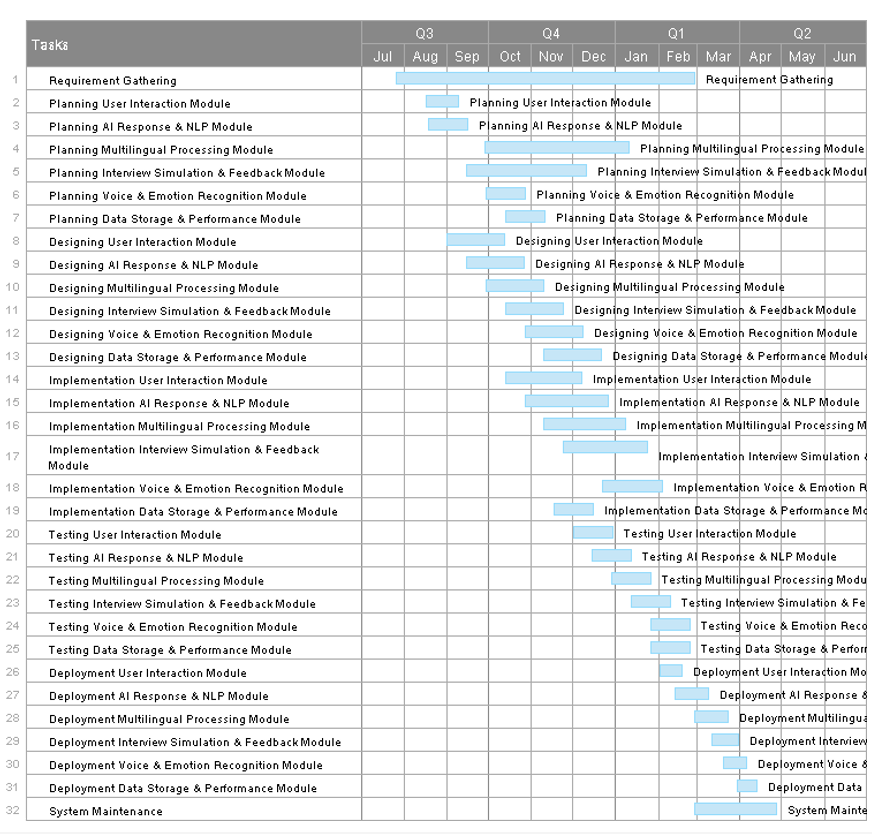
\includegraphics[width=\textwidth]{Gantt New.png}

\vspace{5pt}

\textbf{Figure 4.2: Project Plan (Gantt Chart)}

\end{center}
\vspace{10pt}

\noindent The Figure 4.2 shows the Gantt chart for the development of the Saksham AI – Multilingual AI Interviewer System, which involves several important phases. Initially, the research and planning stage is carried out, where the project requirements are identified and the feasibility of integrating Artificial Intelligence, speech processing, and multilingual capabilities is explored. Following this, the system design phase begins, where the architecture of the AI interviewer platform is structured, including modules such as user interface design, AI-based question generation, response evaluation, and multilingual language processing.
Subsequently, the development phase starts, focusing on implementing the core functionalities of the system such as interview simulation, speech or text interaction, automated feedback generation, and database integration. After development, the testing phase is conducted to verify that the system performs accurately, the interview simulation works smoothly, and the multilingual communication features function effectively.
Once testing is successfully completed, the deployment phase begins, where the system is made available for users to access and practice interview sessions. This phase may also include user guidance or training, helping candidates understand how to interact with the AI interviewer and utilize the feedback system efficiently. Finally, the maintenance phase ensures continuous monitoring, updates, and improvements to maintain system reliability and enhance AI performance. Each phase is carefully represented in the Gantt chart with defined timelines, dependencies, and milestones to ensure systematic development and timely completion of the project.

\vspace{10pt}
\newpage
%------------------------------------------------
% 4.3 Proposed System
%------------------------------------------------

\subsection{Proposed System}

\vspace{10pt}



\begin{center}
\setlength{\fboxsep}{8pt}
\fbox{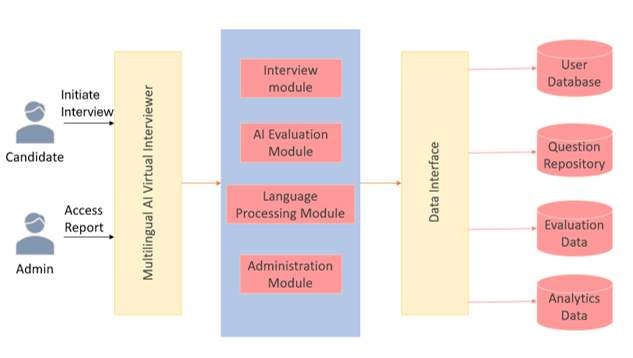
\includegraphics[width=\textwidth]{SYSTEM ARCHI .png}}
\captionof{figure}{Proposed System Architecture of the Multilingual AI Virtual Interviewer System}
\end{center}

\vspace{10pt}
\noindent The Figure 4.3 illustrates the architecture and workflow of the Multilingual AI Virtual Interviewer system, highlighting how various components interact to conduct intelligent, automated, and multilingual interview sessions.

\begin{itemize}

\item The frontend, represented by the Multilingual AI Virtual Interviewer interface, serves as the primary interaction layer for users. It captures requests from candidates initiating interview sessions as well as administrators accessing reports, analytics, or system controls.

\item Upon receiving user input, the frontend forwards the requests to the central backend processing system, which coordinates all core operations and ensures secure and efficient handling of interview activities.

\item The Interview Module manages the complete interview lifecycle, including session initialization, question delivery, response collection, timing control, and progression through the interview stages.

\item The Administration Module supports administrative functions such as report generation, user management, system monitoring, and access control for authorized personnel.

\item The Language Processing Module enables multilingual interaction by performing speech-to-text conversion, language translation, and semantic analysis, allowing candidates to communicate in their preferred language.

\item The AI Evaluation Module analyzes candidate responses using intelligent scoring algorithms and predefined assessment criteria to evaluate communication skills, technical knowledge, and overall performance.

\item The Data Interface functions as the intermediary between application logic and persistent storage, executing CRUD (Create, Read, Update, Delete) operations efficiently while maintaining data integrity and security.

\item Multiple dedicated databases are maintained, including the User Database for profile information, the Question Repository for domain-specific interview questions, Evaluation Data for storing scores and feedback, and Analytics Data for long-term performance insights.

\item The architecture supports real-time data exchange, enabling dynamic question generation, immediate evaluation of responses, and adaptive interview flow based on candidate performance.

\item Processed results and retrieved data are transmitted back to the frontend, updating the user interface instantly to provide a seamless live interview experience for candidates and comprehensive analytical dashboards for administrators.

\end{itemize}
\end{document}